% siminos/presentations/kittens/Bernoulli.tex        pdflatex Bernoulli; biber Bernoulli
% $Author: predrag $ $Date: 2021-12-07 18:54:06 -0500 (Tue, 07 Dec 2021) $

% remember to update \date{December 6, 2021}

                        \newif\ifboyscout\boyscouttrue          %% comments     %%
                        \newif\ifsubmission\submissionfalse     %% internal     %%
                        \newif\ifblog\blogfalse %% section shared with blogCats %%

\input ../../inputs/layoutBeamer
\usepackage[font=scriptsize, labelfont=bf]{caption}
\usepackage[
    backend=biber,  %bibtex,
    sorting=nyt,
    %refsection=chapter,
    %citereset=chapter,
    style=numeric, %alphabetic, % %style=authoryear,
    natbib=true,
    style=phys, % aps
    biblabel= brackets, % superscript, %
    articletitle=false, % true,  % false, % aps
    %chaptertitle=true,  % aip;  % false, % aps
    pageranges = true , % aip: the full range
             % = false, % aps: only the first page being printed
    sortlocale=en_US,
    firstinits=true,
    url=false, %true,  %
    doi=false, %true,
    eprint=false
]{biblatex}
\addbibresource{../../bibtex/siminos.bib}
\setbeamerfont{footnote}{size=\tiny}
%\input ../../inputs/def % no edits, always from dasbuch/book/inputs
\input defsKittens
\input ../../inputs/defsBeamer

\renewcommand{\Ssym}[1]{{\ensuremath{m_{#1}}}}    % Boris
% \newcommand{\Ssym}[1]{{\ensuremath{s_{#1}}}}  % ChaosBook
% \newcommand{\gd}{\mathsf{g}}
\renewcommand{\jacobianOrb}{Hill matrix}
\renewcommand{\JacobianOrb}{Hill matrix}
% \newcommand{\HillDet}{Hill determinant}


\begin{document}
\title{
{\huge what is `chaos'?} %\catlatt}
    \\
{a field theorist stroll through Bernoullistan}
% {\huge Bernoulli  map} %\catlatt}
%    \\
% {essence of deterministic chaos}
}
\author{P. Cvitanovi\'c}
\author[Cvitanovi\'c]
{
  \textcolor{green!50!black}{
  {Predrag~Cvitanovi\'c
%   and
%   Han Liang
%   \\
%  Matt Gudorf,
  }	%\inst{1}
  }
}
\institute
{               Georgia Tech     \\
%  \inst{1}%
%\HREF{https://itsatcuny.org/calendar/chaos-and-quantum-field-theory}
%{ITS Symposium on Chaos and Quantum Field Theory}
    {\scriptsize
 ChaosBook.org/overheads/spatiotemporal \\
 $\to$ Chaotic field theory slides
    }
 }
\date{December 6, 2021}

%\begin{frame}{} %herding cats}
%\begin{center}
%\hfill
\includegraphics[width=0.95\textheight]{DawnBishopCats}
%\end{center}
%\end{frame} %%%%%%%%%%%%%%%%%%%%%%%%%%%%%%%%%%%%%%%%%%%%%%

\begin{frame}
  \titlepage
\end{frame} %%%%%%%%%%%%%%%%%%%%%%%%%%%%%%%%%%%%%%%%%%%%%%

\section[a coin toss]
 {a coin toss}

%%%%%%%%%%%%%%%%%%%%%%%%%%%%%%%%%%%%%%%%%%%%%%%%%%%%%%%%%%
\begin{frame}{}
\begin{bartlett}{
Mephistopheles knocks at Faust's door and says, ``Du
mu{\ss}t es dreimal sagen!"
\\{\color{yellow}.}\qquad
{\scriptsize\emph{``You have to say it three times"}}
        }
\bauthor{
Johann Wolfgang von Goethe
\\{\color{yellow}.}\qquad\quad
{\em Faust I - Studierzimmer 2.~Teil}%\rf{GoetheIstuZim1806}
    }
\end{bartlett}
\vfill
\begin{enumerate}
              \item \textcolor{gray}{\small
\HREF{http://ChaosBook.org/overheads/spatiotemporal/why.pdf}
{what is this about}
                  }
              \item {\Large
\HREF{http://ChaosBook.org/overheads/spatiotemporal/Bernoulli.pdf}
{coin toss}
                  }\textcolor{gray}{\small
              \item
\HREF{http://ChaosBook.org/overheads/spatiotemporal/templatt.pdf}
{\templatt}
              \item
\HREF{http://ChaosBook.org/overheads/spatiotemporal/catlatt.pdf}
{\catlatt}
              \item
\HREF{http://ChaosBook.org/overheads/spatiotemporal/timeDead.pdf}
{bye bye, dynamics}
                    }
            \end{enumerate}
\end{frame} %%%%%%%%%%%%%%%%%%%%%%%%%%%%%%%%%%%%%%%%%%%%%%

\renewcommand{\statesp}{state space}
\renewcommand{\ssp}{\ensuremath{x}}               % state space point

%%%%%%%%%%%%%%%%%%%%%%%%%%%%%%%%%%%%%%%%%%%%%%%%%%%%%%%%%%
\begin{frame}{(1)  coin toss, if you are stuck in XVIII century}
\vfill
    \begin{center}
{\huge time-evolution formulation}
    \end{center}
\vfill
\end{frame} %%%%%%%%%%%%%%%%%%%%%%%%%%%%%%%%%%%%%%%%%%%%%%

%%%%%%%%%%%%%%%%%%%%%%%%%%%%%%%%%%%%%%%%%%%%%%%%%%%%%%%%%%
\begin{frame}{fair coin toss} % ~~~(AKA  }
\renewcommand{\ssp}{\ensuremath{\phi}}             % lattice site field
    \begin{block}{{Bernoulli}  map} %the essence of deterministic chaos}
\begin{center}
            \begin{minipage}[c]{0.36\textwidth}\begin{center}
% ChaosBook {fig:BernPartExam}
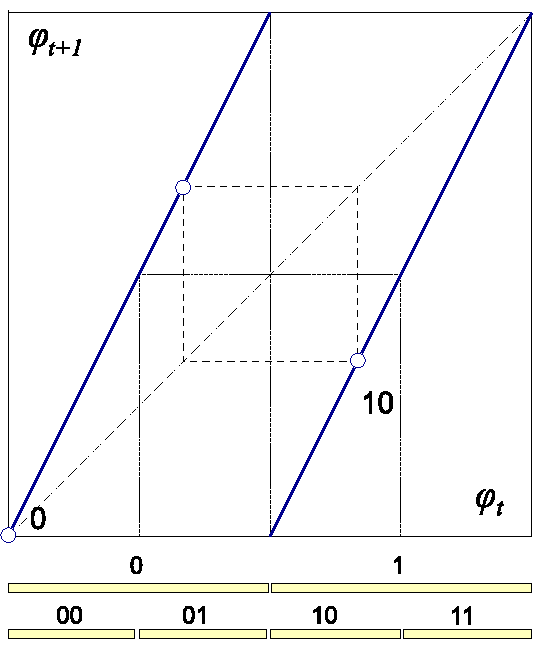
\includegraphics[width=1.0\textwidth]{BernPartKitten}
            \end{center}\end{minipage}
            \hspace{2ex}
            \begin{minipage}[c]{0.46\textwidth}\begin{center}
\[
\ssp_{\zeit+1} =
% \flow{}{\ssp_{\zeit}} =
\left\{ \begin{array}{l} %l}
        % f_0(\ssp_{\zeit}) =
        2 \ssp_{\zeit}
                             \\% \,, \quad & \ssp_{\zeit} \in \pS_0=[0,1/2) \\
        % f_1(\ssp_{\zeit}) =
        2 \ssp_{\zeit} \;\; (\mbox{mod}\;1)
                             % \,, \quad       & \ssp_{\zeit} \in \pS_1 =[1/2,1)
         \end{array}\right.
\]
            \end{center}\end{minipage}
\end{center}
%$\cl{}=2$ and 4 intervals \statesp\ partitions,

\hfill $\Rightarrow$~~~~~
fixed point \cycle{0}, 2-cycle \cycle{01}, $\cdots$
    \end{block}

\bigskip

a \HREF{https://www.random.org/coins/?num=2&cur=40-antique.aurelian}
{coin toss}

\hfill the essence of {\color{blue}deterministic chaos}
\end{frame} %%%%%%%%%%%%%%%%%%%%%%%%%%%%%%%%%%%%%%%%%%%%%%

%%%%%%%%%%%%%%%%%%%%%%%%%%%%%%%%%%%%%%%%%%%%%%%%%%%%%%%%%%
\begin{frame}{what is ({mod}\;1) ?}
\renewcommand{\ssp}{\ensuremath{x}}             % lattice site field
map with integer-valued {\color{blue}`stretching' parameter $s\geq2$} :
\[
\ssp_{\zeit+1} \,=\, {s}\,\ssp_{\zeit}
\] %ee{BerStretch}

$(\mbox{mod}\;1)$ :
subtract the integer part
\(
\Ssym{\zeit}=\left\lfloor{s}\ssp_{\zeit}\right\rfloor
\)

\renewcommand{\ssp}{\ensuremath{\phi}}             % lattice site field
so fractional part
$\ssp_{\zeit+1}$ stays in the unit interval $[0,1)$
\[
\ssp_{\zeit+1}
= {s} \ssp_{\zeit} - \Ssym{\zeit}
\,,\qquad  \ssp_{\zeit}\in\pS_{\Ssym{\zeit}}
\] %ee{circ-m}
$\Ssym{\zeit}$ takes values in the ${s}$-letter alphabet
\[
\Ssym{} \in \A=\{0,1,2,\cdots,s-1\}
\] %ee{base-sAlph}
\end{frame} %%%%%%%%%%%%%%%%%%%%%%%%%%%%%%%%%%%%%%%%%%%%%%

\renewcommand{\ssp}{\ensuremath{\phi}}             % lattice site field
% \renewcommand{\Xx}{\ensuremath{\mathsf{\Phi}}}      % kittens lattice field
\renewcommand{\ssp}{\ensuremath{\phi}}             % lattice site field
% \renewcommand{\Xx}{\ensuremath{\mathsf{\Phi}}}      % kittens lattice field

%%%%%%%%%%%%%%%%%%%%%%%%%%%%%%%%%%%%%%%%%%%%%%%%%%%%%%%%%%
\begin{frame}{a fair dice throw}
    \begin{block}{slope ${6}$ Bernoulli map}
\begin{center}
            \begin{minipage}[c]{0.32\textwidth}\begin{center}
% ChaosBook {fig:BernPartExam}
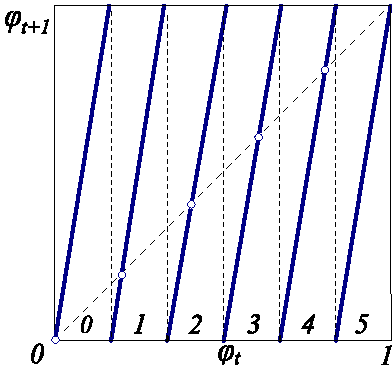
\includegraphics[width=1.0\textwidth]{fig_d_2kitten} % {fig_d_2CL18}
            \end{center}\end{minipage}
            \hspace{2ex}
            \begin{minipage}[c]{0.46\textwidth}
\(
\ssp_{\zeit+1}
= {6} \ssp_{\zeit} - \Ssym{\zeit}
\,,\;  \ssp_{\zeit}\in\pS_{\Ssym{\zeit}}
\)
\medskip

${6}$-letter alphabet \\
\(
\Ssym{\zeit} \in \A=\{0,1,2,\cdots,5\}
\)
            \end{minipage}
\end{center}
$6$ subintervals $\{\pS_{0},\pS_{1},\cdots,\pS_{5}\}$
    \end{block}
\end{frame} %%%%%%%%%%%%%%%%%%%%%%%%%%%%%%%%%%%%%%%%%%%%%%

%%%%%%%%%%%%%%%%%%%%%%%%%%%%%%%%%%%%%%%%%%%%%%%%%%%%%%%%%%
\begin{frame}{what is chaos ?}
    \begin{block}{a fair dice throw}
$6$ subintervals $\{\pS_{\Ssym{\zeit}}\}$,
$6^2$ subintervals $\{\pS_{\Ssym{1}\Ssym{2}}\}, \cdots$
\begin{center}
            \begin{minipage}[c]{0.32\textwidth}\begin{center}
% ChaosBook {fig:BernPartExam}
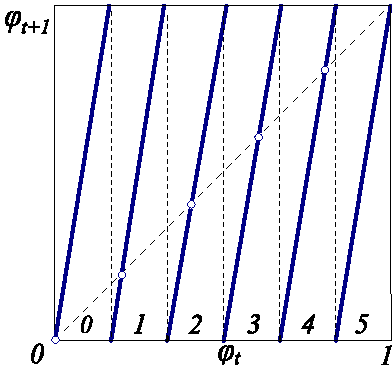
\includegraphics[width=1.0\textwidth]{fig_d_2kitten} % {fig_d_2CL18}
            \end{center}\end{minipage}
            \hspace{2ex}
            \begin{minipage}[c]{0.46\textwidth}
each subinterval contains a periodic point,
labeled by
$\Mm=\Ssym{1}\Ssym{2}\cdots\Ssym{\cl{}}$
\bigskip

$N_\cl{} = 6^\cl{}-1$ {\color{red}unstable} orbits
            \end{minipage}
\end{center}
    \end{block}
\vfill
    \begin{block}{definition : chaos is}
positive Lyapunov $(\ln s)$ - positive entropy $(\frac{1}{\cl{}}\ln N_\cl{})$
    \end{block}
\end{frame} %%%%%%%%%%%%%%%%%%%%%%%%%%%%%%%%%%%%%%%%%%%%%%

%%%%%%%%%%%%%%%%%%%%%%%%%%%%%%%%%%%%%%%%%%%%%%%%%%%%%%%%%%
\begin{frame}{}
    \begin{block}{definition : chaos is}
positive {\color{blue}Lyapunov} $(\ln s)$
         -
positive {\color{blue}entropy} $(\frac{1}{\cl{}}\ln N_\cl{})$
    \end{block}
\bigskip
\begin{itemize}
  \item {\color{blue}Lyapunov} : how fast is local escape?
  \item {\color{blue}entropy} ~~~: how many ways of getting back?
\end{itemize}
                \hfill $\Rightarrow$ {\color{blue}ergodicity}
\vfill
%\hfill
the precise sense in which
\HREF{https://www.random.org/dice/}{dice throw}\\
is an example of deterministic chaos
\end{frame} %%%%%%%%%%%%%%%%%%%%%%%%%%%%%%%%%%%%%%%%%%%%%%

%%%%%%%%%%%%%%%%%%%%%%%%%%%%%%%%%%%%%%%%%%%%%%%%%%%%%%%%%%
\begin{frame}{(2) field theorist's chaos}
\vfill
\begin{center}
{\huge lattice formulation}
\end{center}
\vfill
\end{frame} %%%%%%%%%%%%%%%%%%%%%%%%%%%%%%%%%%%%%%%%%%%%%%

\renewcommand{\Xx}{\ensuremath{\Phi}}

%%%%%%%%%%%%%%%%%%%%%%%%%%%%%%%%%%%%%%%%%%%%%%%%%%%%%%%%%%
\begin{frame}{lattice Bernoulli}
recast the time-evolution Bernoulli map
\[
\ssp_{\zeit+1}
= {s} \ssp_{\zeit} - \Ssym{\zeit}
\] %ee{circ-m}
as 1-step difference equation on the {\color{blue}temporal lattice}
\beq
-\ssp_{\zeit+1} + {s}\ssp_{\zeit} = \Ssym{\zeit}
\,,\qquad  \ssp_{\zeit} \in [0,1)
\ee{1stepDiffEq}
{\color{blue}field} $\ssp_\zeit$, {\color{blue}source} $\Ssym{\zeit}$ \\
on each site $\zeit$ of a
1\dmn\ lattice $\zeit\in\integers$
\bigskip

 write an \cl{}-sites lattice segment as \\
the {\color{blue}field configuration} and the {\color{blue}symbol \brick}
\beq
{\Xx} % = \{\ssp_j\}
             = (\ssp_{\zeit+1},\cdots,\ssp_{\zeit+\cl{}})
\,,\quad
{\Mm} % = \{\Ssym{j}\}
             = (\Ssym{{\zeit+1}},\cdots,\Ssym{{\zeit+\cl{}}})
\ee{pathBern}
`$\Mm$' for `marching orders' ~~:~~ come here, then go there, $\cdots$
\end{frame} %%%%%%%%%%%%%%%%%%%%%%%%%%%%%%%%%%%%%%%%%%%%%%

%%%%%%%%%%%%%%%%%%%%%%%%%%%%%%%%%%%%%%%%%%%%%%%%%%%%%%%%%%
\begin{frame}{scalar  field theory on 1-dimensional lattice}
 write a periodic field over \cl{}-sites Bravais cell as \\
the  {\color{blue}field configuration} and
the {\color{blue}symbol \brick} (sources)
\beq
{\Xx} % = \{\ssp_j\}
             = (\ssp_{\zeit+1},\cdots,\ssp_{\zeit+\cl{}})
\,,\quad
{\Mm} % = \{\Ssym{j}\}
             = (\Ssym{{\zeit+1}},\cdots,\Ssym{{\zeit+\cl{}}})
\ee{pathBern}
\begin{center}
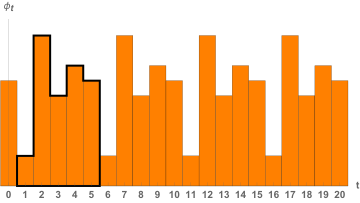
\includegraphics[width=0.85\textheight]{HL1dLatticeStateBar1}
\end{center}

`$\Mm$' for `marching orders' ~~:~~ come here, then go there, $\cdots$
\end{frame} %%%%%%%%%%%%%%%%%%%%%%%%%%%%%%%%%%%%%%%%%%%%%%

%%%%%%%%%%%%%%%%%%%%%%%%%%%%%%%%%%%%%%%%%%%%%%%%%%%%%%%%%%
%\begin{frame}{exponentially many distinct walks through Bernoullistan}
%\begin{center}
%\hfill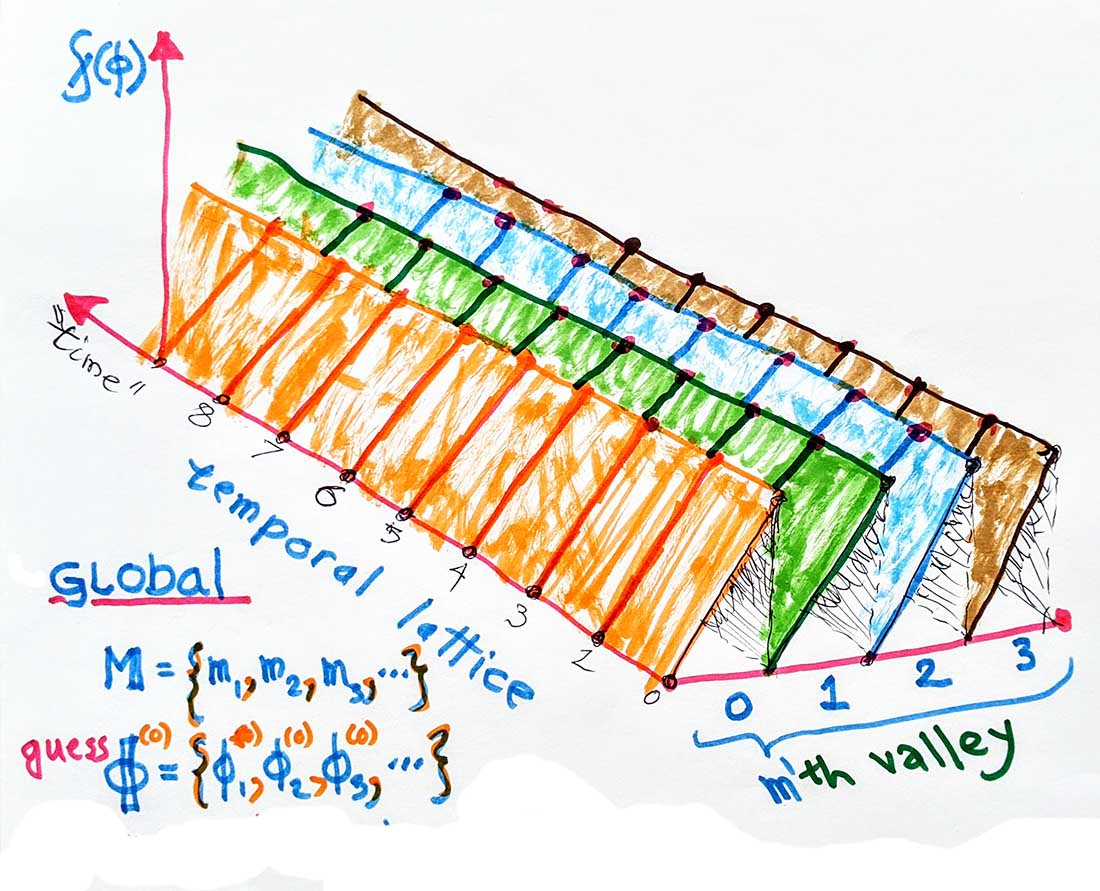
\includegraphics[width=0.90\textwidth]{PC200923Bernoulli1}
%\end{center}
%\end{frame} %%%%%%%%%%%%%%%%%%%%%%%%%%%%%%%%%%%%%%%%%%%%%%


%%%%%%%%%%%%%%%%%%%%%%%%%%%%%%%%%%%%%%%%%%%%%%%%%%%%%%%%%%
\begin{frame}{think globally, act locally}
Bernoulli {\color{blue}condition} at every lattice site $\zeit$,
{\color{blue}local} in time
\beq
-\ssp_{\zeit+1} + {s}\ssp_{\zeit} = \Ssym{\zeit}
\ee{1stepDiffEq}
is enforced by the {\color{blue}global} equation
\beq
\left(-\shift{}+{s}\,\unit\right)\,\Xx =  \Mm
\,,
\ee{tempBern}
$[\cl{}\!\times\!\cl{}]$ shift matrix
\beq
\shift{jk}=\delta_{j+1,k}
\,,\qquad
\shift{}
=  \left(\begin{array}{ccccc}
             0    &  1    &        &   &  \cr
                  &  0    &   1    &   &  \cr
                  &       &        & \ddots &  \cr
                  &       &        & 0 & 1 \cr
             1    &       &        &   & 0
          \end{array} \right)
\ee{hopMatrix}
compares the neighbors
\end{frame} %%%%%%%%%%%%%%%%%%%%%%%%%%%%%%%%%%%%%%%%%%%%%%

%%%%%%%%%%%%%%%%%%%%%%%%%%%%%%%%%%%%%%%%%%%%%%%%%%%%%%%%%%
\begin{frame}{think globally, act locally}
solving the {lattice Bernoulli} system
\[
\jMorb\Xx = \Mm
\,,
\]
$[\cl{}\!\times\!\cl{}]$ {\color{blue}Hill matrix}
~~~~~~~~~~~~~~~
\(
\jMorb = -\shift{}+{s}\,\unit
\,,
\) %{tempBernFix}
\medskip

is a search for zeros of the function
\[
F[\Xx] = \jMorb\Xx - \Mm = 0
\] %{tempFixPoint}
the entire {\color{blue}global lattice state} ${\Xx}_{\Mm}$ is now
\medskip

a single {\color{blue}fixed point}
$(\ssp_1,\ssp_{2},\cdots,\ssp_{\cl{}})$

\hfill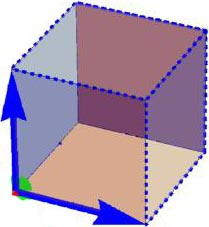
\includegraphics[width=0.12\textwidth]{hyperCube}

\hfill
in the \cl{}\dmn\ unit hyper-cube ~~~~~~~~~~~$\Xx\in[0,1)^\cl{}$
\end{frame} %%%%%%%%%%%%%%%%%%%%%%%%%%%%%%%%%%%%%%%%%%%%%%

%%%%%%%%%%%%%%%%%%%%%%%%%%%%%%%%%%%%%%%%%%%%%%%%%%%%%%%%%%
\begin{frame}{Hill-Poincar\'e}
\vfill
\begin{center}
{\huge orbit stability}
\end{center}
\vfill
\end{frame} %%%%%%%%%%%%%%%%%%%%%%%%%%%%%%%%%%%%%%%%%%%%%%

%%%%%%%%%%%%%%%%%%%%%%%%%%%%%%%%%%%%%%%%%%%%%%%%%%%%%%%%%%
\begin{frame}{\jacobianOrb}
solving a nonlinear
\[
F[\Xx]=0 \quad \mbox{ \color{blue}fixed point condition}
\]
with Newton method requires evaluation of
the $[\cl{}\!\times\!\cl{}]$
    \begin{block}{\jacobianOrb}
\[
\jMorb_{ij} =\frac{\delta F[\Xx]_i}{\delta \ssp_j}
\] %ee{jacobianOrb}
    \end{block}

what does this global \jacobianOrb\ do?
\bigskip

\begin{enumerate}
              \item
fundamental fact {\color{red}!}
              \item
global stability of lattice state \Xx, perturbed everywhere
            \end{enumerate}
\end{frame} %%%%%%%%%%%%%%%%%%%%%%%%%%%%%%%%%%%%%%%%%%%%%%

%%%%%%%%%%%%%%%%%%%%%%%%%%%%%%%%%%%%%%%%%%%%%%%%%%%%%%%%%%
\begin{frame}{(1)}
\vfill
\begin{center}
{\huge fundamental fact}
\end{center}
\vfill
\end{frame} %%%%%%%%%%%%%%%%%%%%%%%%%%%%%%%%%%%%%%%%%%%%%%

%%%%%%%%%%%%%%%%%%%%%%%%%%%%%%%%%%%%%%%%%%%%%%%%%%%%%%%%%%
\begin{frame}{(1) fundamental fact}
to satisfy the fixed point condition
\[
\jMorb\Xx-\Mm = 0
\]
the
 {\jacobianOrb} \jMorb\
\begin{enumerate}
              \item
stretches the unit hyper-cube $\Xx\in[0,1)^\cl{}$ into the \cl{}\dmn\
{\color{blue}\fundPip}
              \item
maps each periodic point ${\Xx}_{\Mm}\;\;\Rightarrow\;\;$ integer lattice
$\integers^\cl{}$ point
              \item
then translate by integers ~~$\Mm\;\;\Rightarrow\;\;$ into the origin
            \end{enumerate}
hence $N_\cl{} =$ total $\sharp$ solutions ~~=~~ $\sharp$
integer lattice points within the {\fundPip}

\bigskip

the {\color{blue}fundamental fact}\footfullcite{BaHePl97} :
{\color{blue}\HillDet} counts solutions
\[
N_\cl{} = \Det\jMorb
\] %ee{detBern0}
$\sharp$ integer points in {\fundPip} $=$ its volume
\end{frame} %%%%%%%%%%%%%%%%%%%%%%%%%%%%%%%%%%%%%%%%%%%%%%

%%%%%%%%%%%%%%%%%%%%%%%%%%%%%%%%%%%%%%%%%%%%%%%%%%%%%%%%%%
\begin{frame}{example : {\fundPip} for $\cl{}=2$}
%$[2\!\times\!2]$

{\jacobianOrb} for ${s} = 2$ ;
unit square basis vectors ;
their images :
\beq
\jMorb =
 \left(\begin{array}{cc}
  2 & -1 \\
 -1 &  2
 \end{array} \right)
;\quad
\Xx_B =
 \left(\begin{array}{c}
 1  \\
 0
 \end{array} \right)
\;\to\;
\Xx_{B'} = \jMorb\,\Xx_B =
 \left(\begin{array}{c}
  2  \\
 -1
 \end{array} \right)
\cdots\,,
\ee{bernFundPar}
%\medskip

    \begin{block}{Bernoulli periodic points of period 2}
    % Predrag 2021-12-05
    % after redefining orbit Jacobian, the figure is wrong, inverted by -1
    % relabel the figure
\begin{center}
            \begin{minipage}[c]{0.32\textwidth}\begin{center}
% ChaosBook {fig:BernPartExam} % BernCyc2Jacob.svg
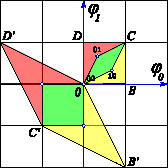
\includegraphics[width=1.0\textwidth]{BernCyc2JacobUnit}
            \end{center}\end{minipage}
            \hspace{2ex}
            \begin{minipage}[c]{0.46\textwidth}
$N_2=3$
\medskip


fixed point ~~$\Xx_{00}$\\
2-cycle ~~~~~~~$\Xx_{01}$, $\Xx_{10}$
            \end{minipage}
\end{center}
    \end{block}
\medskip

square $[0BCD]$
$\Rightarrow\jMorb\Rightarrow$
{\fundPip} $[0B'C'D']$
\end{frame} %%%%%%%%%%%%%%%%%%%%%%%%%%%%%%%%%%%%%%%%%%%%%%

%%%%%%%%%%%%%%%%%%%%%%%%%%%%%%%%%%%%%%%%%%%%%%%%%%%%%%%%%%
\begin{frame}{fundamental fact for any $\cl{}$}

    \begin{block}{an $\cl{}=3$ example} %{\templatt\ $\cl{}=3$ example}
$\jMorb\,$[unit hyper-cube] = [{\fundPip}]
\begin{center}
            \begin{minipage}[c]{0.32\textwidth}\begin{center}
% ChaosBook {fig:BernPartExam} % BernCyc2Jacob.svg
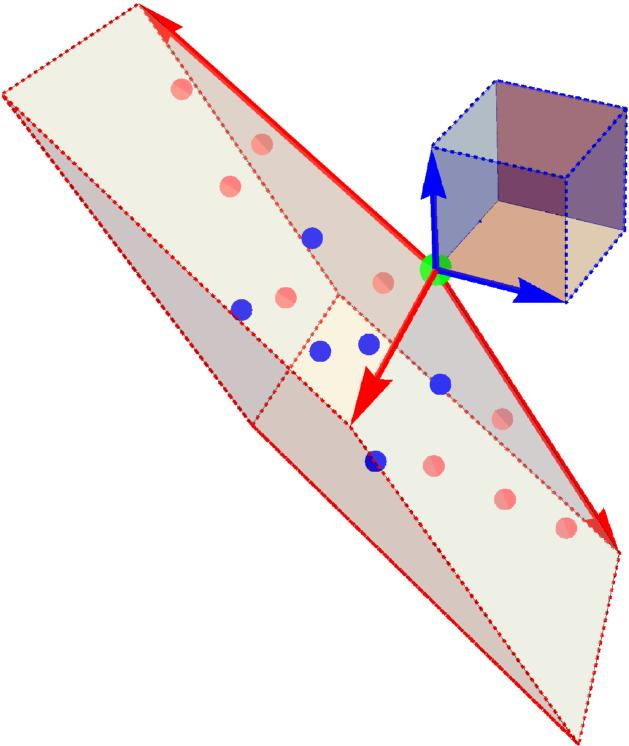
\includegraphics[width=1.0\textwidth]{PCLength3Counting}
            \end{center}\end{minipage}
            \hspace{2ex}
            \begin{minipage}[c]{0.46\textwidth}
unit hyper-cube $\Xx\in[0,1)^3$
\bigskip\bigskip

{\footnotesize $n>3$ cannot visualize}
            \end{minipage}
\end{center}
    \end{block}
    {\footnotesize
a periodic point $\Rightarrow$ integer lattice point :
{\color{red}$\bullet$} on a face,
{\color{blue}$\bullet$} in the interior
    }
\end{frame} %%%%%%%%%%%%%%%%%%%%%%%%%%%%%%%%%%%%%%%%%%%%%%

%%%%%%%%%%%%%%%%%%%%%%%%%%%%%%%%%%%%%%%%%%%%%%%%%%%%%%%%%%
\begin{frame}{(2)}
\vfill
\begin{center}
{\huge orbit stability}
\end{center}
\vfill
\end{frame} %%%%%%%%%%%%%%%%%%%%%%%%%%%%%%%%%%%%%%%%%%%%%%

%%%%%%%%%%%%%%%%%%%%%%%%%%%%%%%%%%%%%%%%%%%%%%%%%%%%%%%%%%
\begin{frame}{(2) orbit stability vs. temporal stability}
\begin{block}{\jacobianOrb}
\(
\jMorb_{ij} =\frac{\delta F[\Xx]_i}{\delta \ssp_j}
\)
stability under {\color{blue}global} perturbation of the whole orbit

\hfill for \cl{} large, a huge $[d\cl{}\!\times\!d\cl{}]$ matrix
\end{block}
\begin{block}{temporal {\jacobianM}}
\(
\jMps%_\Mm
\)
propagates {\color{blue}initial} perturbation $\cl{}$ time steps

\hfill small $[d\!\times\!d]$ matrix
\end{block}
\vfill

$\jMps$ and $\jMorb$ are related by\footfullcite{Hill86}
\begin{block}{Hill's 1886 remarkable formula}
\[
|\Det\jMorb_\Mm| = |\det(\matId - \jMps_\Mm)|
%\label{catHillform}
\]
\end{block}
$\jMorb$ is {\color{red}huge}, even $\infty$\dmn\ matrix\\
$\jMps$ is {\color{red}tiny}, few degrees of freedom matrix
\end{frame} %%%%%%%%%%%%%%%%%%%%%%%%%%%%%%%%%%%%%%%%%%%%%%

%%%%%%%%%%%%%%%%%%%%%%%%%%%%%%%%%%%%%%%%%%%%%%%%%%%%%%%%%%
\begin{frame}{field theorist's chaos}
    \begin{block}{definition : chaos is}
expanding ~~~~~~~~~~~{\color{blue}\HillDet s}
~~~~~~~~~~~$\Det\jMorb$

exponential $\sharp$~~~~~~~~{\color{blue}field configurations}
~~~~~~~$N_\cl{}$~~~
    \end{block}

\bigskip
%\hfill
the precise sense in which

a (discretized) {\color{blue}field theory}
is {\color{blue}deterministically chaotic}

\vfill
 {\color{red}\huge note} : there is
 {\color{red}no} `time' in this definition
\end{frame} %%%%%%%%%%%%%%%%%%%%%%%%%%%%%%%%%%%%%%%%%%%%%%

%%%%%%%%%%%%%%%%%%%%%%%%%%%%%%%%%%%%%%%%%%%%%%%%%%%%%%%%%%
\begin{frame}{}
\vfill
\begin{center}
{\huge \po\ theory}
\end{center}
\vfill
\end{frame} %%%%%%%%%%%%%%%%%%%%%%%%%%%%%%%%%%%%%%%%%%%%%%

%%%%%%%%%%%%%%%%%%%%%%%%%%%%%%%%%%%%%%%%%%%%%%%%%%%%%%%%%%
\begin{frame}{volume of a \po}
Ozorio de Almeida and Hannay\footfullcite{OzoHan84} 1984 :\\
$\sharp$ of periodic points is related to a \JacobianM\ by
\begin{block}{principle of uniformity}
``periodic points of an ergodic system, counted with their natural
weighting, are uniformly dense in phase space''
\end{block}
\bigskip

where
\begin{block}{`natural weight' of \po\ {\Mm}}
\[
  \frac{1}{|\det(\unit - \jMps_{\Mm})|}
\]
\end{block}
\end{frame} %%%%%%%%%%%%%%%%%%%%%%%%%%%%%%%%%%%%%%%%%%%%%%

%%%%%%%%%%%%%%%%%%%%%%%%%%%%%%%%%%%%%%%%%%%%%%%%%%%%%%%%%%
\begin{frame}{\po s partition lattice states into neighborhoods}
how come {\color{blue}\HillDet} $\Det\jMorb$ counts periodic points ?
\bigskip

`principle of uniformity' is in \footfullcite{CBgetused}
\begin{block}{\po\ theory}
known as the \HREF{http://chaosbook.org/chapters/ChaosBook.pdf\#section.27.4} {flow
conservation} sum rule  :
\beq
\sum_{{\Mm}} %\ssp_i{\in\mbox{\footnotesize Fix}\map^{\cl{}}}}
    \frac{1}{|\det (\unit - \jMps_{\Mm})|}
    \;=
\sum_{{\Mm}} %{\ssp_i{\in\mbox{\footnotesize Fix}\map^{\cl{}}}}
    \frac{1}{|\Det\jMorb_{\Mm}|}
    =1
% \label{H-OdeA_mapsOrb}
\eeq
    {\footnotesize
sum over periodic points $\Xx_{\Mm}$ of period \cl{}
    }
\end{block}

\statesp\ is divided into

\hfill
{\color{blue}neighborhoods} of periodic points of period $\cl{}$
\end{frame} %%%%%%%%%%%%%%%%%%%%%%%%%%%%%%%%%%%%%%%%%%%%%%

%%%%%%%%%%%%%%%%%%%%%%%%%%%%%%%%%%%%%%%%%%%%%%%%%%%%%%%%%%
\begin{frame}{\po\ counting}
how come a $\Det\jMorb$ counts periodic points ?
\bigskip

\begin{block}{flow conservation sum rule :}
\[
\sum_{\Xx_\Mm{\in\mbox{\footnotesize Fix}\map^{\cl{}}}}
    \frac{1}{|\Det\jMorb_\Mm|}
    =1
% \label{H-OdeA_mapsOrb}
\]
\end{block}
\medskip

Bernoulli system `natural weighting' is simple :
\medskip

the determinant
$\Det\jMorb_\Mm=\Det\jMorb$ the same for all periodic points, whose
number thus verifies the {\color{blue}fundamental fact}
\[
N_\cl{} = |\Det\jMorb|
\] %ee{detBern0}

\medskip


\vfill
    \begin{block}{the number of Bernoulli periodic lattice states}
\(
N_{\cl{}} = |\Det\jMorb| = s^{\cl{}} - 1
\) %\ee{noPerPtsBm}
~~~~~~~~for any $\cl{}$
    \end{block}
\end{frame} %%%%%%%%%%%%%%%%%%%%%%%%%%%%%%%%%%%%%%%%%%%%%%

%%%%%%%%%%%%%%%%%%%%%%%%%%%%%%%%%%%%%%%%%%%%%%%%%%%%%%%%%%
\begin{frame}{remember the fundamental fact?}
    \begin{block}{period 2 example}
\begin{center}
            \begin{minipage}[c]{0.32\textwidth}\begin{center}
% ChaosBook {fig:BernPartExam} % BernCyc2Jacob.svg
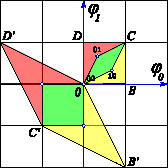
\includegraphics[width=1.0\textwidth]{BernCyc2JacobUnit}
            \end{center}\end{minipage}
            \hspace{2ex}
            \begin{minipage}[c]{0.46\textwidth}
fixed point ~~$\Xx_{00}$\\
2-cycle ~~~~~~~$\Xx_{01}$, $\Xx_{10}$
            \end{minipage}
\end{center}
    \end{block}
\bigskip

$\jMorb\,$[unit hyper-cube] = [{\fundPip}]
\bigskip

look at preimages of the {\fundPip} :
\end{frame} %%%%%%%%%%%%%%%%%%%%%%%%%%%%%%%%%%%%%%%%%%%%%%

%%%%%%%%%%%%%%%%%%%%%%%%%%%%%%%%%%%%%%%%%%%%%%%%%%%%%%%%%%
\begin{frame}{example : lattice states of period 2}
    \begin{block}{unit hypercube, partitioned}
\begin{center}
            \begin{minipage}[c]{0.32\textwidth}\begin{center}
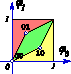
\includegraphics[width=1.0\textwidth]{BernCyc2JacobPart}
            \end{center}\end{minipage}
            \hspace{2ex}
            \begin{minipage}[c]{0.46\textwidth}
fixed point ~~$\Xx_{00}$\\
2-cycle ~~~~~~~$\Xx_{01}$, $\Xx_{10}$
            \end{minipage}
\end{center}
    \end{block}
\medskip

\begin{block}{
\HREF{http://chaosbook.org/chapters/ChaosBook.pdf\#section.27.4} {flow
conservation} sum rule
            }
\beq
      \frac{1}{|\Det{\color{green}\jMorb_{00}}|}
   +    \frac{1}{|\Det{\color{red}\jMorb_{01}}|}
   + \frac{1}{|\Det{\color{yellow}\jMorb_{10}}|}
    =1
% \label{H-OdeA_mapsOrb}
\eeq
    {\footnotesize
sum over periodic points $\Xx_{\Mm}$ of period $\cl{}=2$
    }
\end{block}

\statesp\ is divided into

\hfill
{\color{blue}neighborhoods} of periodic points of period $\cl{}$
\end{frame} %%%%%%%%%%%%%%%%%%%%%%%%%%%%%%%%%%%%%%%%%%%%%%

%%%%%%%%%%%%%%%%%%%%%%%%%%%%%%%%%%%%%%%%%%%%%%%%%%%%%%%%%%
\begin{frame}{}
\begin{center}
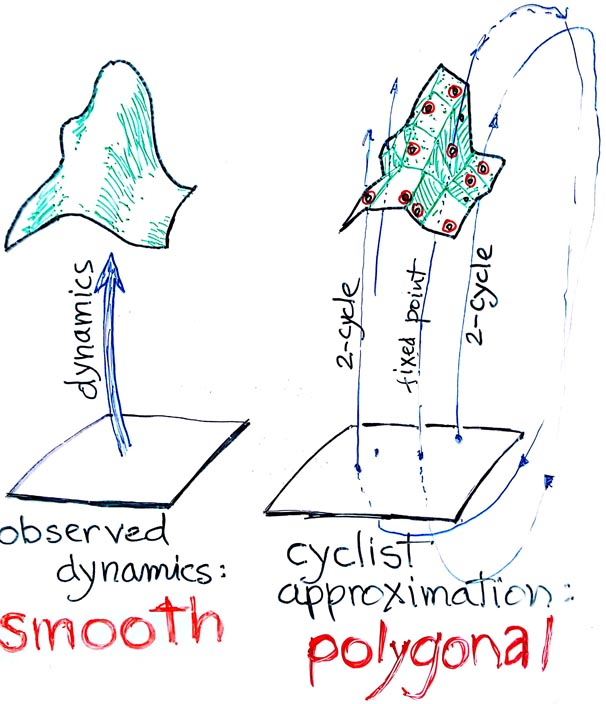
\includegraphics[width=0.60\textwidth]{f_1_08_1}
\end{center}
 tessellate the \statesp\ by {\Large recurrent flows}
\end{frame} %%%%%%%%%%%%%%%%%%%%%%%%%%%%%%%%%%%%%%%%%%%%%%

%%%%%%%%%%%%%%%%%%%%%%%%%%%%%%%%%%%%%%%%%%%%%%%%%%%%%%%%%%
\begin{frame}{}
\begin{bartlett}
     Amazing! I did not understand a single word.
\bauthor{Fritz Haake 1988}
\end{bartlett}

\vfill
\begin{center}
{\huge zeta function}
\end{center}
\vfill
\end{frame} %%%%%%%%%%%%%%%%%%%%%%%%%%%%%%%%%%%%%%%%%%%%%%


%%%%%%%%%%%%%%%%%%%%%%%%%%%%%%%%%%%%%%%%%%%%%%%%%%%%%%%%%%
\begin{frame}{\po\ theory, version (1) : counting {\lattstate}s}

\begin{block}{topological zeta function}
\[
\zetatop(z)
 \,=\,  \exp \left(-\sum_{\cl{}=1}^\infty
\frac{z^\cl{}}{\cl{}} N_\cl{}
         \right)
\] %label{BernZeta}
\end{block}
        \begin{enumerate}
              \item
weight ${1}/{\cl{}}$
as by (cyclic) translation invariance, $\cl{}$ {\lattstate}s are
equivalent
              \item
zeta function counts {\color{blue} orbits}, one per each set of equivalent
{\lattstate}s
            \end{enumerate}
\end{frame} %%%%%%%%%%%%%%%%%%%%%%%%%%%%%%%%%%%%%%%%%%%%%%

%%%%%%%%%%%%%%%%%%%%%%%%%%%%%%%%%%%%%%%%%%%%%%%%%%%%%%%%%%
\begin{frame}{Bernoulli \tzeta}
counts {\color{blue} orbits},
one per each set of {\lattstate}s $N_\cl{}=s^{\cl{}} - 1$
\[
\zetatop(z)
 \,=\,  \exp \left(-\sum_{\cl{}=1}^\infty
\frac{z^\cl{}}{\cl{}} N_n
         \right)
\,=\,
\frac{1 -  {s}z}{1 - z}
\] %label{BernZeta}
numerator $(1 - {s}z)$ says that Bernoulli orbits are built from \\
$s$
fundamental {\color{blue}primitive} {\lattstate}s,

\hfill
the fixed points
$\{\ssp_0,\ssp_1,\cdots,\ssp_{s-1}\}$
\medskip

every other {\lattstate} is
built from their concatenations and repeats.

\vfill
\hfill {\Huge \textcolor{red}{solved!}}
\vfill

{\color{blue}this is `\po\ theory'}
\\
 And if you don't know,
\HREF{https://www.youtube.com/watch?v=_JZom_gVfuw}
{\underline{now you know}}
\end{frame} %%%%%%%%%%%%%%%%%%%%%%%%%%%%%%%%%%%%%%%%%%%%%%

%%%%%%%%%%%%%%%%%%%%%%%%%%%%%%%%%%%%%%%%%%%%%%%%%%%%%%%%%%
\begin{frame}{summary : think globally, act locally}
\bigskip
the problem of enumerating and determining all {\color{blue}{\lattstate}s}
stripped to its essentials :
\bigskip
\begin{enumerate}
              \item
each solution is a zero of the global {\color{blue}fixed point} condition
\[
F[\Xx] = 0
\]
              \item
{\color{blue}global stability} :  the {\jacobianOrb}
\[
\jMorb_{ij} =\frac{\delta F[\Xx]_i}{\delta \ssp_j}
\]
              \item
{\color{blue}fundamental fact} : the number of period-$\cl{}$ orbits
\[
N_\cl{} = |\Det\jMorb|
\]

              \item
{\color{blue}zeta function} $\zetatop(z)$ : all predictions of the theory
            \end{enumerate}
\end{frame} %%%%%%%%%%%%%%%%%%%%%%%%%%%%%%%%%%%%%%%%%%%%%%

%%%%%%%%%%%%%%%%%%%%%%%%%%%%%%%%%%%%%%%%%%%%%%%%%%%%%%%%%%
\begin{frame}{next : a kicked rotor} % - templatt.tex }
\begin{bartlett}{
Du mu{\ss}t es dreimal sagen!
        }
\bauthor{
Mephistopheles
    }
\end{bartlett}
\vfill
\begin{enumerate}
              \item \textcolor{gray}{\small
\HREF{http://ChaosBook.org/overheads/spatiotemporal/why.pdf}
{what is this about}
              \item
\HREF{http://ChaosBook.org/overheads/spatiotemporal/Bernoulli.pdf}
{coin toss}
                  }
              \item {\Large
\HREF{http://ChaosBook.org/overheads/spatiotemporal/templatt.pdf}
{kicked rotor}
                  }\textcolor{gray}{\small
              \item
\HREF{http://ChaosBook.org/overheads/spatiotemporal/catlatt.pdf}
{\catlatt}
              \item
\HREF{http://ChaosBook.org/overheads/spatiotemporal/timeDead.pdf}
{bye bye, dynamics}
                    }
            \end{enumerate}
\end{frame} %%%%%%%%%%%%%%%%%%%%%%%%%%%%%%%%%%%%%%%%%%%%%%

\end{document}
